\chapter{Studie}

\label{AppendixStudie}

\section{Zweck des Dokuments}\label{StudieZweck}

In der Studie werden die Anforderungen aufgenommen, sowie Variantenbeschriebe
für die Projektrealisierung erstellt. Die Varianten werden miteinander
verglichen und durch den Variantenentscheid wird das weitere
Vorgehen definiert.
Ausserdem werden in der Studie die Risiken und Wirtschaftlichkeit des Projekts
analysiert.
\\

\noindent
Folgende Arbeiten werden in dieser Studie abgehandelt:

\begin{itemize}
  \tightlist
  \item der Anforderungskatalog wird definiert
  \item die Evaluation der Browser Software-Technologien
  \item die Evaluation der Server Software-Technologien
  \item die Evaluation der Testing Software-Technologien
  \item eine Kostenschätzung und mögliche Wirtschaftlichkeit ausgerechnet
\end{itemize}


\section{Informationsbeschaffung}\label{informationsbeschaffung}

Folgende Quellen werden in diesem Projekt für die Informationsbeschaffung
genutzt:

\begin{longtable}[]{@{}p{3cm}p{10cm}@{}}
  \toprule
  \textbf{Quelle}               & \textbf{Beschreibung}\tabularnewline
  \toprule
  Schulwissen / Berufserfahrung & Die Grundlage für die Umsetzung dieses Projekts wird durch mein existierendes Schulwissen sowie meine langjährige Berufserfahrung in der Software-Entwicklung gesetzt.\tabularnewline
  \midrule
  Internet                      & Ein Grossteil der Informationen werden heute über das Internet bezogen, für die Evaluation von Technologien und Lösungsansätzen wird einiges über das Internet recherchiert werden müssen.\tabularnewline
  \midrule
  Externer Experte              & Bei konzeptionellen sowie technischen Fragen kann der externe Experte um Rat gefragt werden.\tabularnewline
  \bottomrule
  \caption{Informationsbeschaffung}
\end{longtable}


\clearpage
\section{Anforderungskatalog}\label{anforderungskatalog}

Im Anforderungskatalog werden die Muss- und Kann-Kriterien definiert.
Muss-Kriterien sind zwingend zu erfüllen, Kann-Kriterien sind als optionale
Erweiterung zu verstehen.

% TODO: Fix multirows across pages
%       https://tex.stackexchange.com/questions/79143/how-to-repeat-cell-content-on-next-page-for-longtable-using-multirow/79152
\begin{longtable}[]{@{}p{1.9cm}p{2.5cm}cp{5.5cm}cc@{}}
  \toprule
  \textbf{Feature}           & \textbf{Titel}             & \textbf{Nr.} & \textbf{Kriterium}                                                                                          & \textbf{Ziel} & \textbf{Muss}\tabularnewline
  \midrule
  \endhead
  \multirow{10}{*}{Suche}    & Suche nach Konzertname     & 1.1          & Listet alle Konzerte die Wörter der Suche im Konzertnamen beinhalten                                        & 1.1           & \textbf{Muss}                \\ \cline{2-6}
                             & Suche nach Konzertlocation & 1.2          & Schränkt die Such-Resultate nach gegebener Konzertlocation ein                                              & 1.2           & \textbf{Muss}                \\ \cline{2-6}
                             & Suche nach Ort             & 1.2          & Schränkt die Such-Resultate nach gegebenem Ort ein                                                          & 1.2           & \textbf{Muss}                \\ \cline{2-6}
                             & Suche nach Genre           & 1.2          & Schränkt die Such-Resultate nach gegebenem Musik-Genre ein                                                  & 1.2           & \textbf{Muss}                \\
  \midrule
  \multirow{8}{*}{Design}    & Desktop                    & 2.1          & Alle Ansichten haben eine Desktop-Optimierte Variante                                                       & 1.4           & \textbf{Muss}                \\ \cline{2-6}
                             & Tablet                     & 2.2          & Alle Ansichten haben eine Tablet-Optimierte Variante                                                        & 1.4           & \textbf{Muss}                \\ \cline{2-6}
                             & Mobile                     & 2.3          & Alle Ansichten haben eine Mobile-Optimierte Variante                                                        & 1.4           & \textbf{Muss}                \\ \cline{2-6}
                             & Browser Kompatibilität     & 2.4          & Alle Ansichten müssen in aktuellem Google Chrome und Mozilla Firefox dem Grundlayout folgen                 & 1.9           & \textbf{Muss}                \\
  \midrule
  \multirow{4}{*}{SEO}       & Indexierbarkeit            & 3.1          & Das Produkt ist von Suchmaschinen indexierbar                                                               & 1.5           & \textbf{Muss}                \\ \cline{2-6}
                             & Linked Data                & 3.2          & Konzert Detailseiten sind mit dem Event-Schema\footnote{\url{https://schema.org/Event}} ausgestattet              & 1.5           & \textbf{Muss}                \\
  \midrule
  \multirow{8}{*}{Benutzer}  & Registrierung              & 4.1          & Besucher können sich einen Benutzer registrieren, Benutzernamen und E-Mail Adressen müssen einzigartig sein & 1.6           & \textbf{Muss}                \\ \cline{2-6}
                             & Passwort-Vergessen         & 4.2          & Benutzer können sich einen Passwort-Reset Link anfordern                                                    & 1.7           & \textbf{Muss}                \\ \cline{2-6}
                             & Social                     & 4.3          & Benutzer können auf Konzerten vermerken ob sie Teilnehmen oder nicht                                        & 1.11          & Kann                         \\
  \midrule
  \clearpage
  \multirow{6}{*}{Erfassung} & Artist                     & 5.1          & Benutzer können Artisten mit einem Genre erfassen                                                           & 1.8           & \textbf{Muss}                \\ \cline{2-6}
                             & Location                   & 5.2          & Benutzer können eine Konzertlocation mit Ort/Strasse erfassen                                               & 1.8           & \textbf{Muss}                \\ \cline{2-6}
                             & Konzert                    & 5.3          & Benutzer können ein Konzert mit Konzertlocation und Artisten erfassen                                       & 1.8           & \textbf{Muss}                \\ \cline{2-6}
                             & Facebook                   & 5.4          & Benutzer können ein Konzert in ein Facebook-Event exportieren                                               & 1.10          & Kann                         \\
  \midrule
  \multirow{9}{*}{Security}  & SQL-Injection              & 6.1          & Das Produkt soll resistent gegen SQL-Injection sein                                                         & 1.12          & \textbf{Muss}                \\ \cline{2-6}
                             & HTML-Injection             & 6.2          & Das Produkt soll resistent gegen HTML-Injection / XSS sein                                                  & 1.12          & \textbf{Muss}                \\ \cline{2-6}
                             & Passwort encryption        & 6.3          & Passwörter von Benutzer müssen mit einem sicheren Verfahren gespeichert werden                              & 1.12          & \textbf{Muss}                \\ \cline{2-6}
                             & Session                    & 6.4          & Session-Cookies dürfen nicht durch JavaScript ausgelesen werden                                             & 1.12          & Kann                         \\
  \midrule
  Performance                & Ladezeit                   & 7.1          & Die Seitenansichten dürfen nicht länger als 6 Sekunden auf einem 3G Netz laden                              &               & \textbf{Muss}                \\
  \midrule
  Sonstiges                  & User Tracking              & 8.1          & Benutzerverhalten soll analysiert und nachvollziehbar sein.                                                 &               & Kann                         \\
  \bottomrule
  \caption{Anforderungskatalog}
\end{longtable}


\clearpage
\section{Evaluation Browser-Technologie}\label{evaluation-browser-technologie}

\textbf{Gewichtung:}\\
\textit{5 = Unverzichtbar, 4 = Sehr wichtig, 3 = Erleichtert die Arbeit, 2 = Weniger wichtig, 1 = unwichtig}\\


\begin{longtable}[]{@{}p{2cm}cp{10cm}@{}}
  \toprule
  \textbf{Kriterium} & \textbf{Gewicht} & \textbf{Abnahmekriterium}\tabularnewline
  \midrule
  \endhead
  Komplexität        & 3                & Die Technologie sollte im Rahmen der Diplomarbeit nicht eine zu hohe Komplexität vorweisen. Durch eine niedrigere Komplexität bestehen weniger Risiken dass technische Probleme auftreten werden.\tabularnewline
  \midrule
  Performance        & 4                & In den Projektzielen wurde definiert, dass die Applikation in maximal 6 Sekunden im Browser geladen sein muss. Daher ist es wichtig, dass die Technologie gute Performance Charakteristiken vorweist.\tabularnewline
  \midrule
  SEO                & 5                & Für eine öffentliche Applikation ist es unentbehrlich, dass sie indexierbar durch Suchmaschinen ist.\tabularnewline
  \midrule
  Interaktivität     & 4                & Applikationen im Browser werden immer interaktiver, daher ist es wichtig, das die Technologie anspruchsvolle Abläufe implementieren kann. \tabularnewline
  \midrule
  Stabilität         & 3                & Für das Projekt ist es wichtig, dass auf eine stabile Technologie gesetzt wird, welche den Projektablauf so wenig wie möglich beeinträchtigt. \tabularnewline
  \midrule
  Testing            & 3                & Durch einfaches Testing, kann sichergestellt werden, dass die Applikation wie gewünscht umgesetzt wurde und auch beim Weiterentwickeln nicht existierende Funktionalitäten beinträchtigt werden.\tabularnewline
  \bottomrule
  \caption{Browser-Technologie Kriterien}
\end{longtable}

\clearpage
\subsection{Variante: React}

Die JavaScript Library \textbf{React} ist heute die wohl beliebteste
Technologie um interaktive Applikationen im Web zu bauen.

React ermöglicht es den Entwicklern Screens auf eine deklarative Weise zu
definieren, so dass sich Elemente jeweils dem Zustand der Applikation anpassen.

Die Features von React sind minimal gehalten und sehen auf den ersten Blick
einfach aus, jedoch wird für Anwendungen schnell klar, dass zusätzliche
Software-Libraries benötigt werden um eine grössere Applikation zu entwickeln.

Durch das Hinzufügen von weiteren Libraries steigt die Komplexität dieser
Variante stark an, da es im React Ökosystem für viele Lösungen diverse
verschiedene Lösungsansätze gibt.

\subsection{Variante: Next.js}

\textbf{Next.js} ist ein JavaScript Framework, das auf der \textbf{React}
Library aufbaut und zusätzliche Features sowie gängige Konventionen mitbringt.

Dadurch dass Next.js ein komplettes Framework ist und nicht nur eine Library,
leidet diese Variante weniger der Komplexität eines kompletten Eigenbaus mit
React. Features wie die Navigation von Seite zu Seite bringt Next.js bereits
mit.

\subsection{Variante: SSR}

\textbf{SSR} steht für \textbf{S}erver\textbf{s}ide \textbf{R}endering und
beschreibt die klassische Methode vom Erstellen von Webseiten, indem man HTML
auf dem Server generiert und zum Browser schickt.

Dies hat nach wie vor seine Daseinsberechtigung, da dies wenig Komplexität
mit sich bringt, einen schnelleren Seitenaufbau garantiert und ohne
zusätzlichen Aufwand von Suchmaschinen indexiert werden kann.

\clearpage
\section{Bewertungen Browser-Technologie}\label{bewertungen-browser-technologie}

\textbf{Bewertung:}\\
\textit{4 = Sehr gut, 3 = Gut, 2 = Ungenügend, 1 = Schlecht}\\
\textbf{Gewichtung:}\\
\textit{5 = Unverzichtbar, 4 = Sehr wichtig, 3 = Erleichtert die Arbeit, 2 = Weniger wichtig, 1 = unwichtig}\\


\textbf{\textit{Bewertung x Gewichtung = Punktzahl}}

\begin{longtable}[]{@{}p{2cm}ccccccc@{}}
  \toprule
  \textbf{Kriterium} & \textbf{Gewichtung} & \multicolumn{2}{c}{\textbf{Variante: React}} & \multicolumn{2}{c}{\textbf{Variante: Next.js}} & \multicolumn{2}{c}{\textbf{Variante: SSR}}\tabularnewline
                     &                     & Bewertung                                    & Punkte                                         & Bewertung                                                 & Punkte & Bewertung & Punkte \tabularnewline
  \midrule
  \endhead
  Komplexität        & 3                   & 2                                            & 6                                              & 3                                                         & 9      & 4         & 12 \tabularnewline
  Performance        & 4                   & 3                                            & 12                                             & 3                                                         & 12     & 4         & 16 \tabularnewline
  SEO                & 5                   & 2                                            & 10                                             & 4                                                         & 20     & 4         & 20 \tabularnewline
  Interaktivität     & 4                   & 4                                            & 16                                             & 4                                                         & 16     & 3         & 12 \tabularnewline
  Stabilität         & 3                   & 2                                            & 6                                              & 3                                                         & 9      & 4         & 12 \tabularnewline
  Testing            & 4                   & 4                                            & 16                                             & 4                                                         & 16     & 4         & 16 \tabularnewline
  \midrule
  \textbf{Total:}    &                     & React:                                       & 66                                             & Next.js:                                                  & 82     & SSR:      & 88 \tabularnewline
  \bottomrule
  \caption{Browser-Technologie Bewertung}
\end{longtable}

\section{Entscheid Browser-Technologie}\label{entscheid-browser-technologie}

Durch die Evaluierung wurde klar, dass das Einsetzen eines JavaScript-Frameworks
zuviel zusätzliche Komplexität und gewisse Einbussungen in Performance und Stabilität
unvermeidbar ist. Somit ist ein die Wahl für eine klassische Server-Side Rendered
Webseite favorisierend.

Es ist durchaus vorstellbar, dass in einem zweiten Schritt, nach diesem Projekt,
die Server-Side Rendered Applikation durch eine Next.js Applikation ersetzt werden
könnte.

\subsubsection{Kosten / Wirtschaftlichkeit}

Da die Programmiersprache Elixir sowie das Framework Phoenix unter einer
Open Source Lizenz verfügbar sind, fallen bei dieser Lösung keine zusätzlichen
Kosten an.

\clearpage
\section{Evaluation Server-Technologie}\label{evaluation-server-technologie}

\textbf{Gewichtung:}\\
\textit{5 = Unverzichtbar, 4 = Sehr wichtig, 3 = Erleichtert die Arbeit, 2 = Weniger wichtig, 1 = unwichtig}\\


\begin{longtable}[]{@{}p{2cm}cp{10cm}@{}}
  \toprule
  \textbf{Kriterium} & \textbf{Gewicht} & \textbf{Abnahmekriterium}\tabularnewline
  \midrule
  \endhead
  Komplexität        & 3                & Die Technologie sollte im Rahmen der Diplomarbeit nicht eine zu hohe Komplexität vorweisen. Durch eine niedrigere Komplexität bestehen weniger Risiken dass technische Probleme auftreten werden.\tabularnewline
  \midrule
  Performance        & 4                & In den Projektzielen wurde definiert, dass die Applikation in maximal 6 Sekunden im Browser geladen sein muss. Daher ist es wichtig, dass die Technologie gute Performance Charakteristiken vorweist.\tabularnewline
  \midrule
  Stabilität         & 5                & Während es für die Browser-Technologie vorstellbar ist, die Technologie auszuwechseln, ist es für den Server wichtig auf eine stabile und zukunftssichere Technologie zu setzen.\tabularnewline
  \midrule
  Testing            & 5                & Durch einfaches Testing, kann sichergestellt werden, dass die Applikation wie gewünscht umgesetzt wurde und auch beim Weiterentwickeln nicht existierende Funktionalitäten beinträchtigt werden. Vorallem auf dem Server ist wichtig, dass die Businesslogik gut abdeckend gestestet werden kann.\tabularnewline
  \bottomrule
  \caption{Server-Technologie Kriterien}
\end{longtable}

\subsection{Variante: Node.js / koa.js}

Auch auf dem Server gewinnt JavaScript immer mehr an Beliebtheit.
Mit Node.js und koa.js können schnell kleinere und simplere Applikationen
erstellt werden, die dennoch sehr performant sind.

koa.js ist eine Library für Server-Applikationen und bietet nur eine einfache
Basis und bringt keine Features für Datenpersistenz oder HTML Templates mit sich.
Diese Features müssen durch zusätzliche Module installiert werden.

\subsection{Variante: Elixir / Phoenix}

Elixir ist eine Programmiersprache die eine sehr stabile und performante Grundlage
bietet. Durch das Framework Phoenix, wird im Elixir Ökosystem ein starkes feature
umfangreiches Web-Framework angeboten. Phoenix beinhaltet eine grosse Menge an
Features mit sich und gibt dem Entwickler direkt Funktionalitäten wie HTML
Templates, Datenpersistenz und ein einfaches Test-Framework.

\subsection{Variante: Next.js}

Next.js wurde bereits als Variante für die Browser-Technologie in Betracht
gezogen. Ein zusätzliches Feature von Next.js ist, dass die Applikation auch
auf dem Server betrieben werden kann.
Das Einsetzen der selben Technologie kann bedeutende Vorteile mit sich bringen,
so muss man nur ein Framework lernen und kann Programmcode auf dem Server mit
der Applikation im Browser geteilt werden.

\clearpage
\section{Bewertungen Server-Technologie}\label{bewertungen-server-technologie}

\textbf{Bewertung:}\\
\textit{4 = Sehr gut, 3 = Gut, 2 = Ungenügend, 1 = Schlecht}\\
\textbf{Gewichtung:}\\
\textit{5 = Unverzichtbar, 4 = Sehr wichtig, 3 = Erleichtert die Arbeit, 2 = Weniger wichtig, 1 = unwichtig}\\


\textbf{\textit{Bewertung x Gewichtung = Punktzahl}}

\begin{longtable}[]{@{}p{2cm}ccccccc@{}}
  \toprule
  \textbf{Kriterium} & \textbf{Gewichtung} & \multicolumn{2}{c}{\textbf{Variante: koa.js}} & \multicolumn{2}{c}{\textbf{Variante: Phoenix}} & \multicolumn{2}{c}{\textbf{Variante: Next.js}}\tabularnewline
                     &                     & Bewertung                                     & Punkte                                         & Bewertung                                                     & Punkte & Bewertung & Punkte \tabularnewline
  \midrule
  \endhead
  Komplexität        & 3                   & 2                                             & 6                                              & 4                                                             & 12     & 3         & 9 \tabularnewline
  Performance        & 4                   & 4                                             & 16                                             & 4                                                             & 16     & 3         & 12 \tabularnewline
  Stabilität         & 5                   & 3                                             & 15                                             & 4                                                             & 20     & 3         & 15 \tabularnewline
  Testing            & 5                   & 3                                             & 15                                             & 4                                                             & 20     & 4         & 20 \tabularnewline
  \midrule
  \textbf{Total:}    &                     & koa.js:                                       & 55                                             & Phoenix:                                                      & 68     & Next.js:  & 56 \tabularnewline
  \bottomrule
  \caption{Server-Technologie Bewertung}
\end{longtable}

\section{Entscheid Server-Technologie}\label{entscheid-server-technologie}

Durch das grosse Featurset von Phoenix sowie tieferer Komplexität gegenüber den
beiden anderen Varianten hat sich Phoenix für die Server-Technologie klar
durchgesetzt.

\subsubsection{Kosten / Wirtschaftlichkeit}

Da die Programmiersprache Elixir sowie das Framework Phoenix unter einer
Open Source Lizenz verfügbar sind, fallen bei dieser Lösung keine zusätzlichen
Kosten an.

\clearpage
\section{Evaluation Testing-Technologie}\label{evaluation-testing-technologie}

\textbf{Gewichtung:}\\
\textit{5 = Unverzichtbar, 4 = Sehr wichtig, 3 = Erleichtert die Arbeit, 2 = Weniger wichtig, 1 = unwichtig}\\


\begin{longtable}[]{@{}p{2cm}cp{10cm}@{}}
  \toprule
  \textbf{Kriterium}  & \textbf{Gewicht} & \textbf{Abnahmekriterium}\tabularnewline
  \midrule
  \endhead
  Performance         & 3                & Bei wachsender Anzahl von Tests ist es wichtig, dass die Test-Software genug skalierbar ist um Tests in parallel auszuführen.\tabularnewline
  \midrule
  Stabilität          & 5                & \tabularnewline
  \midrule
  Backend-Integration & 4                & Es ist sehr hilfreich, wenn die End-to-End Test-Software vom Server direkt ausgeführt werden. So kann gleichzeitig zum Browser-Test auch die Businesslogik getestet werden.\tabularnewline
  \midrule
  Visualtesting       & 5                & Die Technologie soll mit dem Service percy.io integrierbar sein.\tabularnewline
  \bottomrule
  \caption{Testing-Technologie Kriterien}
\end{longtable}

\subsection{Jest + Puppeteer}

Jest ist ein JavaScript-Test Framework von Facebook. Durch die Kombinierung der
Puppeteer Library von Google ist es möglich, automatisierte Browser-Tests
durchzuführen.

\subsection{Wallaby}

Wallaby ist ein Elixir Browser-Test Framework, welches sich nahtlos mit Phoenix
integrieren lässt. Wallaby unterstützt parallelisierung von Tests und ist daher
ein guter Kanditat eine hohe Anzahl von automatisierten Tests.

\clearpage
\section{Bewertungen Testing-Technologie}\label{bewertungen-testing-technologie}

\textbf{Bewertung:}\\
\textit{4 = Sehr gut, 3 = Gut, 2 = Ungenügend, 1 = Schlecht}\\
\textbf{Gewichtung:}\\
\textit{5 = Unverzichtbar, 4 = Sehr wichtig, 3 = Erleichtert die Arbeit, 2 = Weniger wichtig, 1 = unwichtig}\\


\textbf{\textit{Bewertung x Gewichtung = Punktzahl}}

\begin{longtable}[]{@{}p{2cm}ccccc@{}}
  \toprule
  \textbf{Kriterium}  & \textbf{Gewichtung} & \multicolumn{2}{c}{\textbf{Variante: Jest}} & \multicolumn{2}{c}{\textbf{Variante: Wallaby}}\tabularnewline
                      &                     & Bewertung                                   & Punkte                                                        & Bewertung & Punkte\tabularnewline
  \midrule
  \endhead
  Performance         & 3                   & 4                                           & 12                                                            & 4         & 12\tabularnewline
  Stabilität          & 5                   & 3                                           & 15                                                            & 4         & 20\tabularnewline
  Backend-Integration & 4                   & 2                                           & 8                                                             & 4         & 16\tabularnewline
  Visualtesting       & 4                   & 4                                           & 16                                                            & 1         & 4\tabularnewline
  \midrule
  \textbf{Total:}     &                     & Jest:                                       & 51                                                            & Wallaby:  & 52\tabularnewline
  \bottomrule
  \caption{Testing-Technologie Bewertung}
\end{longtable}

\section{Entscheid Testing-Technologie}\label{entscheid-testing-technologie}

Dadurch dass sich Wallaby einfach mit der ausgewählten Server-Technologie
verwenden lässt, hohe Performance und Stabilität aufweist, ist Wallaby die
knapp bessere Variante als eine Jest + Puppeteer kombination.

Leider hat Wallaby keine Visualtesting Integration mit dem Dienst percy.io,
dies könnte aber im verlaufe der Umsetzung eventuell im Rahmen dieser Arbeit
umgesetzt werden.

\subsubsection{Kosten / Wirtschaftlichkeit}\label{WallabyPercy}

Auch Wallaby ist unter eines Open Source Lizenz veröffentlicht und erzeugt
somit im Projekt keine direkten zusätzlichen Kosten. Durch fehlende
Unterstützung von Visualtesting, wird im Verlauf der Realisierung zusätzlicher
Aufwand erzeugt, entweder durch eigene Implementation solcher Tests oder durch
unbemerkte Fehler die sich bei Änderungen eingeschlichen haben.

\clearpage
\section{Wirtschaftlichkeit}\label{wirtschaftlichkeit}

\subsection{Projektkosten}

Für die Berechnung der Projektkosten wird ein Stundensatz von 150.- CHF angenommen.

\begin{longtable}[]{@{}lrr@{}}
  \toprule
  \textbf{Phase}  & \makecell[r]{\textbf{Geplante} \\\textbf{Stunden}} & \textbf{Kosten}\tabularnewline
  \midrule
  \endhead
  Initialisierung &  64                       &  9'600.- CHF\tabularnewline
  Konzept         &  66                       &  9'900.- CHF\tabularnewline
  Realisierung    & 136                       & 20'400.- CHF\tabularnewline
  Abschluss       &  64                       &  5'400.- CHF\tabularnewline
  \midrule
  \textbf{Total:} & 286                       & 42'900.- CHF\tabularnewline
  \bottomrule
  \caption{Projektkosten}
\end{longtable}


\noindent
Die geplanten Projektkosten betragen somit \textbf{42'900.- CHF}.

\begin{longtable}[]{@{}lll@{}}
  \toprule
  \textbf{Kostenstelle} & \textbf{Jährliche Kosten}\tabularnewline
  \midrule
  \endhead
  Software              & Keine\tabularnewline
  .com Domain           & 20.- CHF\tabularnewline
  Hosting               & 1'800.- CHF\tabularnewline
  \midrule
  \textbf{Total:}       & 1'820.- CHF\tabularnewline
  \bottomrule
  \caption{Betriebskosten}
\end{longtable}


Für die Betriebskosten eines Hostings wird einen durchschnittlichen monatlichen
Preis von 150.- CHF angenommen, da das Deployment für dieses nicht vorgesehen
ist, ist dies eine von Damian Senn geschätzte Zahl.

\clearpage
\subsection{Break Even Analyse}\label{break-even-analyse}

\subsubsection{Gigboost}

Beim Modell «Gigboost» wird Benutzern eine Option angeboten bei der ihre
publizierten Gigs auf der Startseite sowie in Suchresultaten anderen Einträgen
bevorzugt dargestellt werden. Für einen Gegenpreis von 10.- CHF kann ein Benutzer
seinen Gig «boosten».

\begin{figure}[!htb]
  \centering
  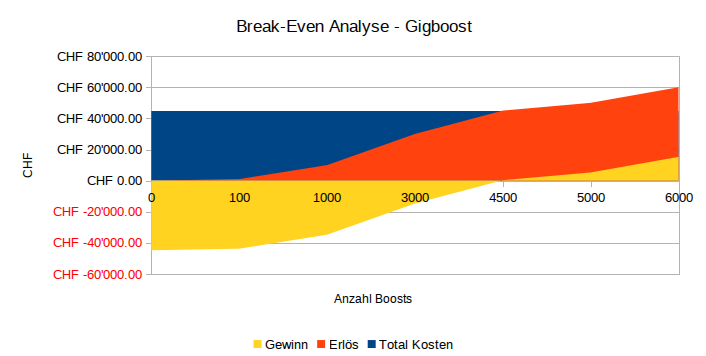
\includegraphics[width=0.95\textwidth]{initialisierung/wirtschaftlichkeit-gigboost.png}
  \caption{Break-Even Analyse - Gigboost}
\end{figure}

\clearpage
\subsubsection{Werbung}\label{break-even-analyse-werbung}

Im Modell «Werbung» wird ausgerechnet wieviele aktive Benutzer das Produkt benötigt
um in den nächsten Jahren Gewinn zu erzielen.

Durch Annahme von einem Erlös von \textbf{140.- CHF} pro \textbf{40'0000 Besucher}\footnote{\url{https://www.quora.com/How-much-does-Google-AdSense-pay-for-3-banners-on-a-webpage-per-1-000-views/answer/Manas-Sahu-59}} erhalten wir folgendes Bild:

\begin{figure}[!htb]
  \centering
  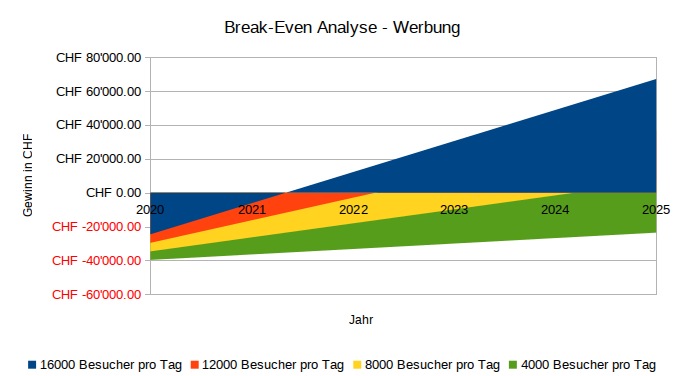
\includegraphics[width=0.95\textwidth]{initialisierung/wirtschaftlichkeit-werbung.png}
  \caption{Break-Even Analyse - Werbung}
\end{figure}

\begin{longtable}[]{@{}lll@{}}
  \toprule
  \textbf{Besucher pro Tag} & \textbf{Erlös pro Tag} & \textbf{Erlös pro Monat}\tabularnewline
  2'000                     & 7.- CHF                & 210.- CHF\tabularnewline
  4'000                     & 14.- CHF               & 420.- CHF\tabularnewline
  8'000                     & 28.- CHF               & 840.- CHF\tabularnewline
  12'000                    & 42.- CHF               & 1'260.- CHF\tabularnewline
  16'000                    & 46.- CHF               & 1'680.- CHF\tabularnewline
  \bottomrule
  \caption{Werbeeinnahmen pro Besucher}
\end{longtable}

Der Grafik ist zu entnehmen, dass das Produkt bei 8'000 Besucher pro Tag nach ca. 6 Jahren Gewinn erzielt. Bei 12'000 Besucher pro Tag erzielt das Produkt nach bereits 4 Jahren Gewinn und mit 16'000 Beucher pro Tag schon im dritten Jahr.

